\chapter{Application to Estimation of Data Dimension}

\section{Chernoff-Okamoto Inequality}

Let $X_i$ be a sample from the Bernoulli distribution $\Be(p)$. Define $ X = \sum_{i = 1}^n X_i$, and let $\lambda = np = \E X$. 
Note that for $u > 0$, 
  \begin{equation}\label{co:1}
    \everymath{\displaystyle}\arraycolsep=1.4pt\def\arraystretch{1.5}
  \begin{array}{l}
    \E e^{uX} = \prod_i \E e^{uX_i} = {((1-p) + p e^{u})}^n,\\
    \E e^{-uX} = \prod_i \E e^{-uX_i} = {((1-p) + p e^{-u})}^n.
  \end{array} 
  \end{equation}
  By applying Markov's Inequality to $e^{uX}$, we can assert that
  \[\everymath{\displaystyle}\arraycolsep=1.4pt\def\arraystretch{1.5}
  \begin{array}{rcl}
    \P\{X \geq \lambda + t\} & = & \P\{e^{uX} \geq e^{u(\lambda + t)}\}\\
    & \leq & e^{-u(\lambda+t)} \cdot \E e^{uX}\\
    & = & e^{-u(\lambda+ t)} \cdot {(1-p + p e^{u})}^n. 
  \end{array} \] 
  According to~\cite{janson2002concentration}, the right hand equation is minimized when,
  \[ e^{u} = \frac{\lambda+t}{(n-\lambda-t)} \cdot \frac{1-p}{p}. \]
  Therefore, for $0 \leq t \leq n-\lambda$,
  \begin{equation}\label{co:2}
    \P\{X \geq \lambda + t\} \leq {\left(\frac{\lambda}{\lambda+t}\right)}^{\lambda + t} {\left(\frac{n-\lambda}{n-\lambda-t}\right)}^{n - \lambda - t}.
  \end{equation}

  However, a simpler expression is required for the following application.

\begin{theorem}\label{co:T1}
  Let $X$ be the random variable we defined at the start of this chapter. In particular, $X$ is a random variable with the binomial distribution $\Bi(n,p)$ with $\lambda := np = \E X$, then for $t \geq 0$,
  \begin{equation}\label{co:3}
    \P\{X \leq \lambda - t\} \leq \exp\left(- \frac{t^2}{2\lambda}\right).
  \end{equation}
\end{theorem}

\textbf{Used in:} Theorem~\ref{ade:T2}

\begin{proof}
This proof was adapted from Appendix A.1.13 from~\cite{alon2016probabilistic}. The first step is to apply formula~\ref{co:1}
  \[ 
    \everymath{\displaystyle}\arraycolsep=1.4pt\def\arraystretch{1.5}
    \begin{array}{rcl}
      \P \{X < \lambda - t\} & = & \P \{e^{-uX} < e^{-u(\lambda - t)}\}\\
      & \leq & e^{u(\lambda-t)} \E e^{-uX}\\
      & = & e^{u(\lambda-t)} e^{u\lambda} {((1-p) + p e^{-u})}^n.
    \end{array} 
   \]
   Then, use the inequality $1+u\leq e^{u}$ to conclude,
   \[ (1-p)+pe^{-u} = 1+(e^{-u}-1)p < e^{p(e^{-u}-1)} \]
   \[ \implies {((1-p)+pe^{-u})}^n \leq e^{np(e^{-u}-1)} = e^{\lambda(e^{-u}-1)}. \] 
   Combining everything, we obtain
   \[ \P \{X < \lambda - t\} \leq e^{\lambda(e^{-u}-1)+\lambda u - ut} \]
   Now, we employ the following inequality obtained by the Taylor series expansion,
   \[ e^{-u} \leq 1-u+u^2/2.\]
   After expanding, this results in 
   \[ \P \{X < \lambda - t\} \leq e^{\lambda u^2 / 2 - ut}. \]
   Finally, by replacing $u = t/\lambda$ we obtain the desired result:
   \[ \P \{X < \lambda - t\} \leq e^{-t^2/2\lambda}. \] 
\end{proof}

\section{The problem}

The article~\cite{diaz2019local} explains how we can estimate the dimension $d$ of a manifold $M$ embedded on a Euclidean space of dimension $m$, say $\R^m$. First, we are going to introduce the method they used, and then, we will show how the exponential inequalities can be used to prove two important results in the paper. The procedure starts with an example on a uniformly distributed sample on a $d$-sphere $\S^{d-1} \subset \R^d$, but will be later generalized for samples of any distribution with a density bounded away from zero.\\[1em]

In the first place, let $Z_1, \ldots, Z_k$ be a i.i.d.\ sample uniformly distributed on $\S^{d-1}$. Then, we have the following formula for the variance of the angles between $Z_i,Z_j, i\neq j$:

\begin{equation}\label{ade:1}\everymath{\displaystyle}
  \beta_d := \Var(\arccos \angles{Z_i,Z_j}) = \begin{cases}
    \frac{\pi^2}{4} - 2 \sum_{j = 1}^{k} {(2j-1)}^{-2}, & \mbox{ if } d = 2k+1 \mbox{ is odd},\\
    \frac{\pi^2}{12}- 2 \sum_{j = 1}^{k} {(2j)}^{-2}, & \mbox{ if } d = 2k+2 \mbox{ is even.}
  \end{cases}
\end{equation}

The previous formula for the angle variance is proven in~\cite{diaz2019local}. In order to give more insight on how we will be choosing an estimator $\widehat{d}$ of the dimension of the sphere, consider the following theorem.

\begin{theorem}[Bounds for $\beta_d$]\label{ade:T1}
  For every $d > 1$,
  \[ \frac{1}{d} \leq \beta_d \;\leq\; \frac{1}{d-1}. \] 
\end{theorem}
\begin{proof}[]

\end{proof}

\vspace*{1em}

Knowing that for every $d > 1$, $\beta_d$ is in the interval $[\tfrac{1}{d}, \tfrac{1}{d-1}]$, one can guess the dimension of the sphere by estimating $\beta_d$, and then, taking $d$ from the lower bound of the interval where our estimator is. Since $\beta_d$ is the variance of the angles in our sphere, our best choice for an estimator is the angle's sample variance,


\begin{equation}\label{ade:2}
  U_{k} = \binom{k}{2}^{-1} \sum_{i<j\leq k}{\left(
    \arccos\angles{Z_i, Z_j} - \frac{\pi^2}{2} 
    \right)}^{2}.
\end{equation}

In Proposition 1.\ of~\cite{diaz2019local} the authors prove that it's the Minimum Variance Unbiased Estimator for $\beta_d$ on the unit sphere.\\[0.5 em]

Furthermore, the authors also prove that there are some conditions on a manifold and on the data sampling distribution for which this result can be generalized. Let $X_1,\ldots, X_n$ be a i.i.d.\ sample from a random distribution $P$ on a manifold $M \subset \R^m$, and let $p \in M$ denote a point on the manifold. For $C>0 \in  \R$, let $k = \ceil{C \ln(n)}$ and define $R(n) = L_{k+1}(p)$ as the distance between $p$ and its $(k+1)$-nearest neighbor. W.L.O.G. assume that $p = 0 \in M$ and that $X_1,\ldots, X_k$ are the $k$-nearest neighbors of $p$. Additionally, for the following theorems to be true, we have the following requirements:

\begin{itemize}
  \item The distribution of the sample has a continuous density.
  \item The density at every point of any neighborhood of $p$ is positive.
  \item The manifold is at least twice differentiable. 
\end{itemize}

The following theorem uses a special inequality from Chernoff-Okamoto, and it's crucial in the idea behind this generalization.

\begin{theorem}[Bound $k$-neighbors]\label{ade:T2}
  For any sufficiently large $C > 0$, we have that, there exists $n_0$ such that, with probability 1, for every $n \geq n_0$,
  \begin{equation}\label{ade:3}
    R(n) \leq f_{p,P,C}(n) = O(\sqrt[d]{\ln(n)/n}),
  \end{equation}
  where the function $f_{p,P,C}$ is a deterministic function which depends on $p,\, P$ and $C$.
\end{theorem}

\begin{proof}[]

\end{proof}

\vspace*{0.5 em}

The following theorem, although it does not require concentration inequalities, is important for connecting the idea of the previous theorem to the main frame. Let $\pi : \R^m \to T_p M$ denote the orthogonal projection on the Tangent Space of $M$ at $p$. Also, define $W_i := \pi(X_i)$ and then normalize,
\begin{equation}\label{ade:4}
  Z_i := \frac{X_i}{\|X_i\|},\hspace*{5mm} \widehat{W_i} := \frac{W_i}{\|W_i\|}.
\end{equation}

\begin{theorem}[Projection Distance Bounds]\label{ade:T3}
  For any $i<j \leq n$,
  \begin{enumerate}
    \item[(i)]    \( \|X_i-\pi(X_i)\|  =   O(\|\pi (X_i)\|^2). \hfill\inlinetag  \)
    \item[(ii)]   \( \|Z_i-\widehat{W_i}\|  =   O(\|\pi (X_i) \|). \hfill\inlinetag \)
    \item[(iii)]  The difference between inner products (cosine of angles) can be bounded as follows:
    \begin{equation}\label{ade:7}
      |\angles{Z_i,Z_j} - \langle\widehat{W_i}, \widehat{W_j}\rangle| \leq C r,
    \end{equation}
    for a constant $C\in\R$, whenever $r \geq \max (\|\pi(X_i)\|,\|\pi(X_j)\|)$.
  \end{enumerate}
\end{theorem}
\begin{proof}[]

\end{proof}

\vspace*{0.5 em}

What follows is that if we know $W_1,\ldots, W_k$ are behaved similar to a uniformly distributed sample on the sphere $\S^d$, then, $Z_1,\ldots, Z_k$ (the normalized $k$-nearest neighbors of $p$) also behave like they are uniformly distributed on $\S^d$. The following theorem is made by combining the ideas of the previous theorems.

\begin{theorem}[Projection's Angle Variance Statistic]\label{ade:T4}
  For $k = O(\ln n)$, let
  \begin{equation}\label{ade:8}
    V_{k,n} = \binom{k}{2}^{-1} \sum_{i<j\leq k}{\left(
      \arccos\angles{\widehat{W_i}, \widehat{W_j}} - \frac{\pi^2}{2} 
      \right)}^{2},
  \end{equation}
  and let $U_{k,n} = U_k$ from equation~\ref{ade:2}. The following statements hold
  \begin{enumerate}
    \item[(i)]    \( k |U_{k,n} - V_{k,n}| \overset{n\to\infty}{\longrightarrow} 0,\;\mbox{in probability}. \hfill\inlinetag  \)
    \item[(ii)]    \( \E |U_{k,n} - V_{k,n}| \overset{n\to\infty}{\longrightarrow} 0\).
  \end{enumerate}
\end{theorem}
\begin{proof}[]

\end{proof}

\vspace*{0.5 em}

This last theorem is as far as this document is planned to cover. However, the last result in the paper provides the main statement. It says that if we estimate $\beta_d$ as we did with $U_{k,n}$ from~\ref{ade:T4}, and then, extract $\widehat{d}$ from the interval where $U_{k,n}$ is located, it follows that,
\begin{theorem}[Consistency]\label{ade:T5}
  When $n\to \infty$,
  \[ \P\{\widehat{d} \neq d\} \to 0.\]
\end{theorem}

\section{Proofs}

\begin{proof}[Proof Theorem~\ref{ade:T1}:]\label{ade:T1P}
  The even and the odd cases must be distinguished:
  \begin{enumerate}
    \item[(1):] When $d = 2k+2$ is even:
    In the first place, remember that,
    \[ \lim_{k\to\infty}\; \sum_{j = 1}^{k} j^{-2} = \frac{\pi^2}{6}.\] 
    It follows from the equation~\ref{ade:1} that
    \[\everymath{\displaystyle}\arraycolsep=1.8pt\def\arraystretch{1.8}
      \begin{array}{rrlll}
        \beta_d & = & \frac{\pi^2}{12} - 2 \sum_{j = 1}^{k} {(2j)}^{-2}= & \frac{\pi^2}{12} - \frac{1}{2} \sum_{j = 1}^{k} j^{-2}\\
        & = & \frac{1}{2} \sum_{j = k+1}^{\infty} j^{-2}.
      \end{array}      
     \]
    Since ${(j^{-2})}_{j \in \N}$ is a monotonically decreasing sequence, it follows that
    \[\everymath{\displaystyle}\arraycolsep=1.5pt\def\arraystretch{1.5}
      \begin{array}{rrcll}
        \frac{1}{d}   & = & \frac{1}{2k+2}  & = & \frac{1}{2} \int_{k+1}^{\infty}x^{-2} dx\\[5mm]
      & \leq & \beta_d  & \leq & \frac{1}{2} \int_{k+1/2}^{\infty}x^{-2} dx\\[5mm]
      & = & \frac{1}{2k+1} & = & \frac{1}{d-1}.
    \end{array}  \] 

    \item[(2):] When $d = 2k+3$ is odd:
    On the other hand, note that
    \[\hspace{-35mm}\everymath{\displaystyle}\arraycolsep=1.5pt\def\arraystretch{1.5}
      \begin{array}{rcl}
      \lim_{k\to\infty} \; \sum_{j = 1}^{k} {(2j-1)}^{-2} 
      & = & \lim_{k\to\infty} \sum_{j = 1}^{2k-1} j^{-2} - \sum_{j = 1}^{k-1} {(2j)}^{-2}\\
      & = & \lim_{k\to\infty} \sum_{j = 1}^{2k-1} j^{-2} - \frac{1}{4}\sum_{j = 1}^{k-1} j^{-2}\\
      & = & \frac{\pi^2}{6}-\frac{\pi^2}{24} = \frac{\pi^2}{8}.
    \end{array}\]
    Hence,
    \[\hspace{-10mm}\everymath{\displaystyle}\arraycolsep=1.5pt\def\arraystretch{1.5}
    \begin{array}{rll}
      \beta_d & = & \frac{\pi^2}{4} - 2 \sum_{j = 1}^{k} {\left(2j-1\right)}^{-2}\\
      & = & 2\sum_{j = k+1}^{\infty}{\left(2j-1\right)}^{-2}.\\
    \end{array}      
   \]
   Using a similar argument we conclude that
   \[\everymath{\displaystyle}\arraycolsep=1.5pt\def\arraystretch{1.5}
      \begin{array}{rrcrl}
        \frac{1}{d} & = & \frac{1}{2k+1}  & = & 2 \int_{k+1}^{\infty}{(2x-1)}^{-2} dx\\[5mm]
      & \leq & \beta_d    & \leq & 2 \int_{k+1/2}^{\infty}{(2x-1)}^{-2} dx\\[5mm]
      &  = & \frac{1}{2k+2} & = & \frac{1}{d-1}.
    \end{array}  \] 
  \end{enumerate}
\end{proof}

\begin{proof}[Proof Theorem~\ref{ade:T2}:]\label{ade:T2P}

The volume of a $d$-sphere of radius $r$ is equal to:

\[ v_d r^d = \frac{\pi^{d/2}}{\Gamma(\tfrac{n}{2}+1)} r^d, \]

where $v_d$ is the volume of the unit $d$-sphere. For the assumptions we made on $P$ and $M$ around $p = 0$, we can say that for any $r > 0$, there's a percent (greater than 0) of the sample that is within a range $r$ from $p$. This proportion is subordinated only by the volume of a $d$-sphere of radius $r$ and a constant $\alpha := \alpha(P)$ that depends on the distribution $P$:

\[ \rho = \P\{X \in M : |X| < r\} \geq \alpha v_d r^d  > 0.  \] 

We can now define a binomial process based on how many neighbors does $p$ have within a range $r$. Let $N = N_r \sim \Bi(n,\rho)$ be the number of neighbors, using Theorem~\ref{co:T1} with $\lambda = n\rho $ and $t = \tfrac{\lambda}{2}$ we obtain,

\[ \P\{N \leq \lambda - t\} = \P\{2N \leq \lambda \} \leq \exp(-\lambda/8). \] 

Since $n(\alpha v_d r^d) \leq n\rho = \lambda$, it follows that, by choosing $r(n)$ such that 
\[ \tag*{($\star$)} r(n) = {\left(\frac{C}{\alpha v_d} \cdot \frac{\ln n}{n} \right)}^{1/d} = O(\sqrt[d]{\ln(n)/n}),\]
and thus,
\[ C \ln n = n(\alpha v_d r{(n)}^d) \leq \lambda,\]
we obtain:
\[P\{2N \leq C \ln n \} \leq \P\{2N \leq \lambda \}, \]
and,
\[\exp(-\lambda/8)  \leq  \exp\left(\frac{-C\ln n}{8}\right) = n^{-C/8}.\]
Therefore, if $C > 8$, then
\[P\{2N \leq C \ln n \} \leq  n^{-C/8},\]
which implies, from the same argument using Borel Cantelli~\ref{borel-cantelli} in chapter 2, that this probability converges to 0. Finally, with this last expression we proved that if $k = \tfrac{C}{2}\ln n$, then the $k$-neighbors of $p$ are contained in the ball of radius $r(n)$ with a probability that converges exponentially to 1.
\end{proof}

\begin{proof}[Proof Theorem~\ref{ade:T3}:]\label{ade:T3P}
  W.L.O.G. we assumed from the beginning that $p=0$ by translating everything. Let $(U, x_1, \ldots, x_m)$ be a chart for $p \in M$. Since the real dimension of the manifold is $d$, there exists by Theorem 11.5~\cite{tu2011manifolds}, a change of basis $(U, z_1, \ldots, z_m)$ such that $T_p M$ is spanned by $\angles{z_1,\ldots, z_d}$.
  
  \vspace*{1em}
  
  Let $\pi : M \to T_p M$ be the projection from $M$ to its tangent space at $p$. This function is differentiable and its derivative at $p$ is the identity. Therefore, by the Implicit Function Theorem, there exists a neighborhood $V \subset \R^m$ of $p$ such that $\pi |_{V\cap M}$ is a diffeomorphism and that there exists a chart $(V\cap T_p M, \phi)$ defined as follows:
  
  \[ \phi : V\cap T_p M \to M,\] 

  \begin{equation}\label{ade:phi}
    \phi(z_1, \ldots, z_d) = (z_1,\ldots, z_d, F_1(z_1,\ldots, z_d),\ldots, F_{t}(z_1,\ldots, z_d)),
  \end{equation}
  
  with $t = m-d$, $\phi(0) = p = 0$ and $\partial F(p)/ \partial z_j = 0$ for $i \leq t$ and $j \leq d$. Then, the distance between a point in $V\cap M$ and its projection is expressed in the local coordinates as follows,

  \[ \text{f}(z) = \text{dist}((z,0,\ldots,0) - \phi(z)) = \sqrt{F_1^2(z)+ \cdots + F_t^2(z)}. \]
  Now, Taylor's theorem stats that at $p$, the distance function,

  \[ \text{f}(z) = f(p) + df(p) \cdot (z-p) + \sum_{i = 2}^{\infty} g_i(p) {(z-p)}^i. \]
  Since $p = 0$, then ${(z-p)}^i = \|z\|^2 {(z)}^{i-2}$ for $i \geq 2$. Also,

  \[ f(p) = \text{dist}((0,\ldots, 0)- \phi(0)) = 0, \]
  Also, $df(p) = 0$ because the partial derivatives of $F_j$ are 0, and since the tangent space is a linear approximation of $M$ at $p$, the rate of change of the error between a point in $M$ and its projection at $T_p M$ should go to 0 when we are close to $p$. Thus,

  \[ \text{f}(z) = \cancelto{0}{f(p)} + \cancelto{0}{df(p)} \cdot z + \|z\|^2 \sum_{i = 2}^{\infty} g_i(p) z^{i-2}. \]
  Since $\lim_{i\to\infty} g_i(p) = 0$, it follows that there exists $G \in \R$ such that $G = \max |g_i(p)|$
  Assume without lose of generality that $V \subset B_{1/2}(0)$. It follows that for $z \in V\cap T_p M$,
  \[ \everymath{\displaystyle}\arraycolsep=1.4pt\def\arraystretch{1.5} 
  \begin{array}{rcl}
    \text{f}(z) & \leq & \|z\|^2 \sum_{i = 0}^{\infty} |g_i(p)| \cdot \|z\|^i\\
    & \leq & \|z\|^2 \cdot \frac{G}{1-\|z\|}\\
    \text{\scriptsize ($\|z\| \leq 2$)}\hspace*{0.5em} & = & 2G\|z\|^2 = K\|z\|^2.
  \end{array} \] 

  This proves that there exists a constant $K$ for which $\|X - \pi X\| \leq K \|X\|^2$ for $X$ very close to $p$, which proves equation 3.2.5.


  \[ \left\| \frac{X}{\|\pi X\|} - \frac{\pi X}{\|\pi X\|} \right\| \leq K\|\pi X\|. \]
  
  \[ \everymath{\displaystyle}\arraycolsep=1.4pt\def\arraystretch{1.5}
  \begin{array}{rcl}
    \left\| \frac{X}{\|X\|} - \frac{X}{\|\pi X\|} \right\| & = & \|X\| \left| \frac{1}{\|X\|} - \frac{1}{\|\pi X\|} \right|\\
    & = & \Big|\|X\|- \|\pi X\|\Big| \cdot \|\pi X\|^{-1}\\
    & \leq & \|X-\pi X\|\cdot\|\pi X\|^{-1}\\
    & \leq & K \|\pi X\|.
  \end{array}
  \] 

  By plugging everything together, we obtain

  \[ \|Z - \widehat{W}\| = \left\|\frac{X}{\|X\|} - \frac{\pi X}{\|\pi X\|}\right\| \leq  {\left\| \frac{X}{\|X\|} - \frac{X}{\|\pi X\|} \right\|} + { \left\| \frac{X}{\|\pi X\|} - \frac{\pi X}{\|\pi X\|} \right\|} \leq 2 K \|\pi X\|.\] 

  This proves equation 3.2.6. 3.2.7 follows immediately from 3.26 and the triangle inequality.
  
\end{proof}

\begin{proof}[Proof Theorem~\ref{ade:T4}:]\label{ade:T4P} 
For every $ i\leq k$, from the way we parametrized the tangent space in equation~\ref{ade:phi}, it's clear that $\|\pi X_i\| \leq \|X_i\| \leq R(n)$:

\vspace*{1em}

  \begin{center}
  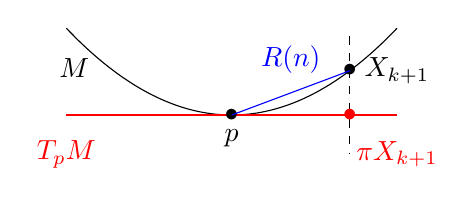
\begin{tikzpicture}
    % \draw[->] (-2.4, 0) -- (2.4, 0) node[right] {};
    \draw[scale=1, domain=-2.1:2.1, smooth, variable=\x, black] plot ({\x}, { (\x/2)^2+1});
    \draw[scale=1, domain=-2.1:2.1, smooth, variable=\y, red]  plot ({\y}, {1}); % Divided \x and \y by 2 on the 2nd coordinate to scale the y axis by 1/2.
        \node[text=black] at (-2,1.6) {$M$};
    \node[text=red] at (-2.1,0.5) {$T_p M$};
    \draw [dashed] (1.5, 2) -- (1.5,0.5);
    \node[text=black] at (0,1) {$\bullet$};
    \node[text=black] at (0,0.7) {$p$};
    \node[text=black] at (1.5,{(1.5/2)^2 + 1}) {$\bullet$};
    \node[text=black] at (2.1,{(1.5/2)^2 + 1}) {$X_{k+1}$};
    \node[text=red] at (1.5,1) {$\bullet$};
    \node[text=red] at (2.1,0.5) {$\pi X_{k+1}$};
  
    \draw[blue] (0, 1) -- (1.5, {(1.5/2)^2 + 1});
    \node[text=blue] at (0.75,1.7) {$R(n)$};
  \end{tikzpicture}
\end{center}

  \vspace*{1em}

  Then, from theorems~\ref{ade:T2} and~\ref{ade:T3}.\text{(ii)} it follows that
  \[ \max_{i \leq k} \|Z_i - \widehat{W}_i\| = O_\P (r(n)) = O_\P [{(\ln n / n)}^{1/d}].\] 
  Thus,
  \[ \max_{i \leq k} |\angles{Z_i,Z_j} - \langle\widehat{W}_i, \widehat{W}_j\rangle| = O_\P (r(n)). \]
  Now, in order to continue, we must prove the following inequality.
  \begin{lemma}
    For $c_1, c_2 \in [-1, 1]$ such that $c_2-c_1 \leq 1/4$, we have
    \[ |\arccos(c_2) - \arccos(c_1)| \leq 2 \sqrt{|c_2 - c_1|}. \] 
  \end{lemma}

  \begin{proof}
    Assume W.L.O.G. that $c_2 \geq c_1$. If $c_1,c_2 > 0$, then
    \[ \everymath{\displaystyle}\arraycolsep=1.4pt\def\arraystretch{2}
    \begin{array}{rcl}
      |\arccos(c_2) - \arccos(c_1)| & = & \int_{c_1}^{c_2} {(1-x^2)}^{-1/2}dx\\
      & \leq & \int_{1-(c_2-c_1)}^{1} {(1-x^2)}^{-1/2}dx\\
      \text{\scriptsize ($ u = 1-x $)}\hspace*{0.5em} & = & \int_0^{c_2-c_1} {(2u-u^2)}^{-1/2}\\
      & \leq & \int_0^{c_2-c_1} u^{-1/2} du\\
      & = & 2 \sqrt{|c_2 - c_1|}.
    \end{array}
    \]

    This argument is identical in the case where $c_2, c_1$ are both negative. If $c_2 \geq 0$ and $c_1 \leq 0$, then $c_2, c_1 \in [-1/4, 1/4]$. Since $\arccos$ is monotonically decreasing and its derivative is bounded in this interval, by the mean value theorem there exists $t\in \R$ such that
    \[\everymath{\displaystyle}\arraycolsep=1.4pt\def\arraystretch{1.5} 
      \begin{array}{rcl}
      |\arccos(c_2)-\arccos(c_1)| & = & (c_2-c_1) \frac{1}{\sqrt{1-t^2}}\\
      & \leq & |c_2-c_1| \sup_{x \in [-1/4, 1/4]} \frac{1}{\sqrt{1-x^2}}\\
      & = & |c_2-c_1| \sqrt{\frac{4}{3}} \\
      \text{\scriptsize ($x \leq 1/4 \implies x \leq \sqrt{x} $)}\hspace*{0.5em}  & \leq & 2 |c_2-c_1| \leq 2 \sqrt{|c_2 - c_1|}.
    \end{array} \] 
  \end{proof}
  From the previous lemma we obtain,
  \[ \begin{array}{rcl}
    \max_{i< j \leq k} \left|\arccos\angles{Z_i,Z_j} - \arccos\angles{\widehat{W}_i,\widehat{W}_j}\right| & \leq & \sqrt{\max_{i \leq k} |\angles{Z_i,Z_j} - \langle\widehat{W}_i, \widehat{W}_j\rangle|}\\
    & = & O_\P(\sqrt{r(n)}). 
  \end{array}\] 
  The lemma is also true for values under the application $u\mapsto {(u-\pi)}^2$ because this function is Lipschitz near $p = 0$, so it follows that, after taking the expected value on each side,
  \[ U_{k,n} - V_{k,n} = O_\P(\sqrt{r(n)}) = O_\P [{(\ln n / n)}^{1/(2d)}] .\]
  Therefore, for $k = C \ln(n)$,
  \[ k \cdot O_\P [{(\ln n / n)}^{1/(2d)}] = o_{\P}(1),\]
  which proves part (i). Part (ii) follows from the fact that $ U_{k,n} - V_{k,n}  $ is a bounded random variable whose probability converges to 0. Thus, its expected value also converges to 0.
\end{proof}